\documentclass{article}
\usepackage{graphicx}

\usepackage{amsmath}

\begin{document}

\begin{center}
	Inverted pendulun on a cart
\end{center}

\begin{figure}[h]
	\centering
	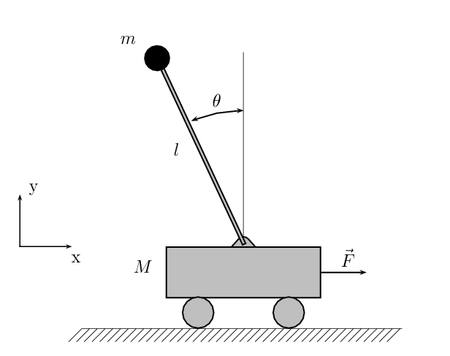
\includegraphics[scale=2]{Cart-pendulum.png}
\end{figure}

Lagrange equations:

\begin{eqnarray}
	\frac{d}{dt}\frac{\partial L}{\partial \dot{\theta}}-\frac{\partial L}{\partial \theta}=0,\\
	\frac{d}{dt}\frac{\partial L}{\partial \dot{x}}-\frac{\partial L}{\partial x}=F.
\end{eqnarray}
where
\begin{eqnarray}
	L=\frac{1}{2}(M+m)\dot{x^2}-ml\dot{x}\dot{\theta}\cos\theta +\frac{1}{2}ml^2\dot{\theta}^2-mgl\cos\theta.
\end{eqnarray}

Resulting dynamics equations:

\begin{eqnarray}
	\left\{
		\begin{aligned}
		& (m+M)\ddot{x}-ml\ddot{\theta}\cos\theta+ml\dot{\theta}^2sin\theta = F,\\
		& l\ddot{\theta}-g\sin\theta = \ddot{x}\cos\theta.
		\end{aligned}
	\right.
\end{eqnarray}

State vector

\begin{eqnarray}
\left\{
\begin{aligned}
& theta,\\
& \omega = \dot{\theta},\\
& x,\\
& v =\dot{x}.
\end{aligned}
\right.
\end{eqnarray}

State vector derivative

\begin{eqnarray}
\left\{
\begin{aligned}
& \dot{\theta}=\omega,\\
& \dot{\omega}=\frac{g\sin\theta+mF/(m+M)-l\dot{\theta}^2\cos\theta\sin\theta m/(m+M)}{l-l\cos^2\theta m/(m+M)},\\
& x,\\
& \dot{x}=\frac{F+mg\cos\theta\sin\theta+ml\dot{\theta}^2\sin\theta}{m+M-m\cos^2\theta}.
\end{aligned}
\right.
\end{eqnarray}
	
\end{document}